\section{Problems 2 and 3. Exact search on a finite score table}
\subhead{One representative of each metal site}
Let $a_i,b_j\in\{0,1\}$ indicate the selected A and B elements. For Q2 let $C_{ij}=\Vh(i,j,\noo)$. For Q3 store
\begin{equation}
 C_{ij}=\min_{x\in\{\ooo,\noo,\foo\}}\Vh(i,j,x),
 \qquad x^*_{ij}\in\arg\min_x\Vh(i,j,x).
 \label{eq:envelope}
\end{equation}
Taking $\min_{ij}$ in Eq.~\eqref{eq:envelope} visits every eligible triple. Recover $x^*_{ij}$ after choosing the pair, taking the smallest official ID in a tie. A joint one-hot encoding has 156 choices of $(A,X)$ and 52 choices of B. Eliminating X leaves 104 binary variables and a 2,704-cell table. It requires all 8,112 scores in advance. Solving three separate fixed-X problems is another exact decomposition.

For either real cost table, let $D$ denote its min--max normalization. The exactly-one penalty formulation \cite{lucas} is
\begin{equation}
 E(a,b)=\sum_{ij} D_{ij}a_i b_j+
 P\left[\left(\sum_i a_i-1\right)^2+\left(\sum_j b_j-1\right)^2\right].
 \label{eq:qubo}
\end{equation}
Each legal vector activates one cell. Each illegal vector has penalty at least $P$ and nonnegative table cost, so $P>1$ separates it from every legal state before rounding. The encoding represents any predictor evaluated on this finite pool. Requiring the fitted predictor itself to be quadratic would impose an unnecessary restriction.

\subhead{What changes at eight bits?}
Kaiwu converts linear fields to couplings with a reference spin, producing 105 Ising dimensions. The special-purpose quantum computer (SPQC) interface specifies signed 8-bit integer couplings \cite{sdk}. We convert Eq.~\eqref{eq:qubo} to Ising, apply the SDK precision adjustment at eight bits, convert back, and compare energies of all 2,704 legal states. We scan $P=1.1,3,10$ using the full Q3 envelope and a version capped at its tenth percentile before normalization. Both tables have the same original minimizer. Figure~\ref{fig:precision} compares the excess score on the unrounded table at each setting.

\begin{figure}[htbp]
\centering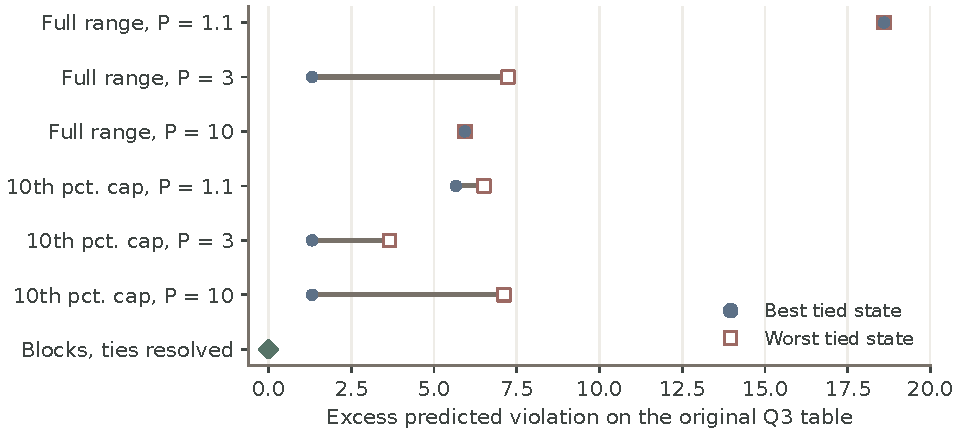
\includegraphics[width=.92\linewidth]{figures/precision.pdf}
\caption{Q3 original-score excess among legal states minimizing each quantized whole-grid energy. A segment spans tied outcomes. Coincident endpoints indicate identical excess. The diamond gives the verified result of the block method.}\label{fig:precision}
\end{figure}

\section{An eight-bit encoding with a checkable minimum}
All six whole-grid configurations in Figure~\ref{fig:precision} lose the minimum of the frozen mixture. For the full range and $P=1.1$, the winning legal pair costs an extra 18.5949 units of $\Vh$. A cap and $P=3$ reduce the best tied excess to 1.3175, still above zero. This audit checks only legal states. We now construct smaller blocks whose entire unconstrained state spaces can be checked.

Sort A and B alphabetically and partition each into thirteen consecutive groups of four. Each of the resulting 169 blocks $T$ covers 16 pairs. Let $M=\max_{ij\in T} C_{ij}$. For nonnegative costs use
\begin{equation}
 q_{ij}=\operatorname{round}(15C_{ij}/M),\quad
 q_{ij}\in\{0,\ldots,15\},\qquad P=16. \label{eq:bins}
\end{equation}
If $M=0$ set the whole block to zero. Use $q$ in Eq.~\eqref{eq:qubo}. A legal state has energy at most 15, whereas every illegal state costs at least 16. Rounding is monotone: the original block minimum is among the rounded minima. Retrieve the complete set of tied minima, read their original costs and keep the least. Comparing the 169 retained original costs recovers the global minimum. This proof depends on retrieving every ground state in a tied block. A sampler returning one arbitrary optimum has a weaker guarantee.

\subhead{Why the coefficients fit}
Write the upper-triangular QUBO with diagonal $-16$, within-group interactions $32$ and cross-group interactions $q_{ij}$, omitting the common constant 32. For eight bits $z$, set $s=2z-1$ and use one reference spin. With Kaiwu's $-s^\mathsf{T}Js$ convention, multiplying the returned symmetric matrix by eight gives integral couplings. Within-group entries are $-32$, cross-group entries are $-q_{ij}$. Each reference coupling is
\begin{equation}
 -\left(2(-16)+3(32)+\sum_{k=1}^4 q_{ik}\right)
 =-\left(64+\sum_{k=1}^4 q_{ik}\right), \label{eq:refcoupling}
\end{equation}
using the corresponding column sum on the B side. Equation~\eqref{eq:refcoupling} bounds its magnitude by 124. This is an a priori 8-bit bound for every block, independent of the absolute units of $\Vh$.

Kaiwu's \texttt{BruteForceOptimizer} solves the resulting nine-spin instances on the local CPU. We fix the gauge by multiplying every spin by the reference spin and deduplicate binary states. An independent pass checks all $2^8=256$ assignments in each block, including infeasible assignments. It verifies the affine energy relation, counts ground states, and compares every decoded optimum with the integer-cost table. Across both pools all 338 calls return complete sets of feasible ground states. Every retained block winner also matches the minimum of its original floating-point block.

\subhead{Why use four elements on each side?}
For a block of $n$ rows and $n$ columns with integer costs in $[0,K]$, the reference coupling of one logical variable has magnitude bounded by
\[
 B(n,K,P)=2P(n-2)+nK,\qquad n\geq2 .
\]
The $n-1$ same-register partners each contribute $2P$ and the diagonal contributes $-2P$ inside the reference term. Each of the $n$ cross-register partners contributes at most $K$. With $P=16$, $K=15$, blocks of side three, four and five have respective bounds 77, 124 and 171. Four is the largest uniform side length guaranteed to fit signed eight-bit couplings under this integer scaling. A particular five-element block may fit if its row and column sums are small. The uniform construction eliminates that data-dependent assumption.
\subsection{A worked example of an integer-energy tie}
Consider a Q3 block whose rows are Ir, K, La and Li and whose columns are Ge, Hf, Hg and In. In Figure~\ref{fig:tile} we select this block because, among the 169 Q3 blocks it has the largest spread of original scores tied at the lowest integer cost. It illustrates the cost of returning a single arbitrary ground state when the solver can return the whole tied set.

\begin{figure}[htbp]
\centering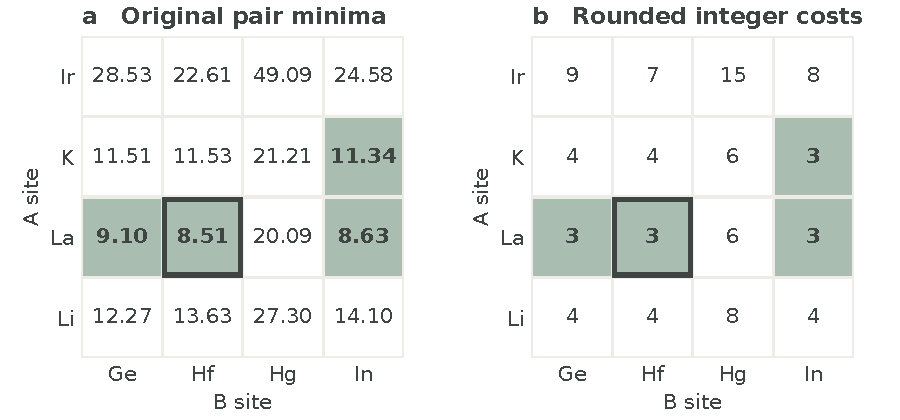
\includegraphics[width=.91\linewidth]{figures/tied_block.pdf}
\caption{The same Q3 block before and after Eq.~\eqref{eq:bins}. Shaded, bold cells share the lowest integer cost. The dark outline marks La--Hf, the original minimum. K--In ties after rounding but has an original score 2.82808 units higher. Displayed raw costs are rounded to two decimals after the calculation.}\label{fig:tile}
\end{figure}

The largest score in this block is 49.089358. The spacing of one integer bin is consequently about $49.089358/15=3.2726$ score units. Four pairs occupy the lowest bin. Their original scores are 8.511569 for La--Hf, 8.629274 for La--In, 9.102727 for La--Ge and 11.339649 for K--In. Each pair already carries its own minimizing $X$ from Eq.~\eqref{eq:envelope}. Selecting K--In would sacrifice 2.828081 units despite reaching the same minimum integer energy. Reading back the four original values returns La--Hf.

This example explains the difference between feasibility and selection accuracy. The penalty $P=16$ certifies one A and one B for every ground state in this block. It cannot distinguish the four shaded cells in Figure~\ref{fig:tile}. The monotonicity argument only places the best real-valued candidate somewhere among them. Full ground-state retrieval plus the original-score comparison is the additional condition needed for equality with the floating-point block minimum.

Integer minima tie in 70 of 169 Q3 blocks and 71 of 169 Q2 blocks. Choosing the highest original score among tied minima in every block gives the same two global winners in these runs because each winning block has a single minimizer. The largest within-block losses under this rule are 2.828081 for Q3 and 3.013807 for Q2. The cost breakdown includes time spent decoding and resolving ties.

\section{Selected compositions and computational cost}
Table~\ref{tab:answers} reports the single selections for Q2 and Q3 and the corresponding blind-pool checks.
\begin{table}[htbp]
\caption{Answers and membership checks. The two full pools are solved by Kaiwu. Direct scans of the two blind subsets give the restricted-pool comparison.}\label{tab:answers}
\centering\small\begin{tabular}{llrllrr}
\toprule Task & Pool (size) & ID & $(A,B,X)$ & Formula & $\Vh$ & Public $V$\\\midrule
Q2 & 07 (2,704)&13153& La, Ti, NO2 & LaTiO$_2$N & 6.924382 & hidden\\
Q3 & 08 (8,112)&8760& Sn, Ti, O3 & SnTiO$_3$ & 3.268113 & 0.001419\\\midrule
Q2 & 11 (529)&13153& La, Ti, NO2 & LaTiO$_2$N & 6.924382 & hidden\\
Q3 & 12 (1,587)&13153& La, Ti, NO2 & LaTiO$_2$N & 6.924382 & hidden\\\bottomrule
\end{tabular}
\end{table}
All four winners use the same refitted model. The ordered triplets explain why the file's NO2 family is written as O$_2$N in the supplied formula. For Q2 and Q3, respectively, runner-up scores are 7.256664 and 3.904881. Enumeration gaps for the chosen records are zero. Their winning-block Ising energies under $-s^\mathsf{T}Js$ are $-702$ and $-724$. Constants and scales vary by block, so comparing those two energies would have no physical meaning. $\mathrm{SnTiO_3}$ belongs to file 02; its public value is an in-training observation after refitting. For a new DFT calculation in the blind pool, both objectives nominate $\mathrm{LaTiO_2N}$. The appendix compares its three anion choices (Figure~\ref{fig:families}).

\subhead{Reading the selected bits}
A low Ising energy becomes a material recommendation only after the binary state has been decoded and compared across blocks. Figure~\ref{fig:decode} follows the Q3 winner. Holding Sn and Ti fixed, the three family scores are 3.2681 for O3, 8.2041 for FO2 and 12.3445 for NO2. The envelope stores the first value together with the O3 family and original row ID 8760.

\begin{figure}[htbp]
\centering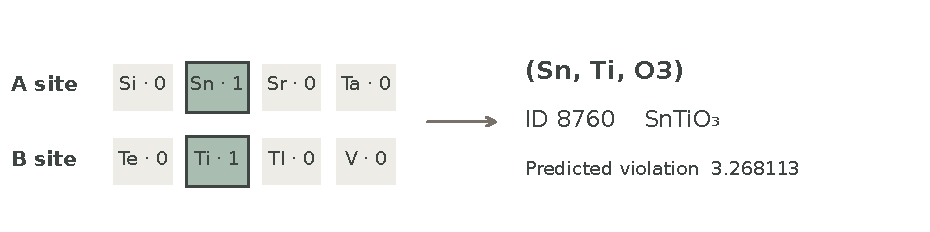
\includegraphics[width=\linewidth]{figures/qubo_decode.pdf}
\caption{Readout of the winning Q3 block. Each register contains exactly one active bit. Combining Sn and Ti with the stored minimizing family returns the full-pool material shown in Table~\ref{tab:answers}.}\label{fig:decode}
\end{figure}

The ordering $(\mathrm{Si,Sn,Sr,Ta})$ on A and $(\mathrm{Te,Ti,Tl,V})$ on B makes the second bit active in each register. If $\sigma_i$ is a returned spin and $\sigma_r$ the reference spin, the implemented readout is
\[
 z_i=\tfrac12(1+\sigma_i\sigma_r).
\]
Simultaneously reversing every spin leaves every product unchanged. The two gauge representations therefore identify the same pair and should be counted once. Fixing the reference to $+1$ gives binary vectors $(0,1,0,0)$ on both sides. The winning state's measured SDK energy is $-724$ and the decoded raw score is 3.268113. The block's lowest integer cost has one legal pair. Other blocks have different scale factors and omitted constants; their winners enter the final comparison through their raw scores.


Table~\ref{tab:cost} separates shared fitting and scoring costs from the pool-specific solver and scan times.

\begin{table}[htbp]
\caption{Wall-clock measurements on an AMD Ryzen 9 8945HX CPU. Fitting the three-component model is shared across both optimization problems.}\label{tab:cost}
\centering\small\begin{tabular}{lrr}
\toprule Stage & Q2 & Q3\\\midrule
Descriptors, shared (s) & \multicolumn{2}{c}{\DescFull}\\
Refit on 15,225 rows, shared (s) & \multicolumn{2}{c}{\FitFull}\\
Score 8,112 rows, shared (s) & \multicolumn{2}{c}{\ScoreFull}\\
Subset, index and reduce pool (s) & \PoolTwo & \PoolThree\\
Construct and convert 169 blocks (s) & \EncodeTwo & \EncodeThree\\
169 Kaiwu CPU solves (s) & \SolveTwo & \SolveThree\\
Decode, resolve ties, verify (s) & \CheckTwo & \CheckThree\\
Direct array minimum, median ($\mu$s) & \ScanTwo & \ScanThree\\
Blocks with ties / 169 & \TiedTwo & \TiedThree\\
Original costs compared within tied or unique minima & \FinalistsTwo & \FinalistsThree\\
Observed integer coupling range & $[\CoeffLowTwo,0]$ & $[\CoeffLowThree,0]$\\\bottomrule
\end{tabular}
\end{table}
The direct scan uses the same in-memory predictions and times 1,001 repetitions of one array minimum. The larger QUBO times include the checks itemized above; disk I/O and manuscript generation lie outside these timings. For Q1 alone, descriptors, training and scoring the hidden set took \DescOne, \FitOne\ and \ScoreOne\ seconds. These are local wall times under the observed machine load. Device programming, queueing, sampling, energy consumption and hardware success rates remain unmeasured.

\subsection{How much score error can change the recommendation?}
Checking the original score after decoding certifies the winner for a frozen table. Its robustness to changes in that table can be computed separately. Let $s_1<s_2$ denote the first two scores in one specified pool. If each score changes by at most $\epsilon$, the original winner remains strictly first whenever
\begin{equation}
 s_1+\epsilon<s_2-\epsilon
 \quad\Longleftrightarrow\quad \epsilon<(s_2-s_1)/2 .
 \label{eq:margin}
\end{equation}
The condition is sharp under independent bounded perturbations. Opposite changes at the two leading entries can create a tie at equality. If changes are correlated by composition, this worst case may be unattainable. Table~\ref{tab:margins} applies Eq.~\eqref{eq:margin} to each frozen pool. The resulting radii bound changes in predicted scores.

\begin{table}[htbp]
\caption{Selection margins in the archived Q2/Q3 refit. The last column counts records, including the winner, with predicted score at most two units above the minimum.}\label{tab:margins}
\centering\small\begin{tabular}{llrrr}
\toprule Pool & Runner-up & $s_2-s_1$ & Half-margin & Within 2 units\\\midrule
Q2 full (07) & $\mathrm{YTiO_2N}$ & 0.332282 & 0.166141 & 5\\
Q2 blind (11) & $\mathrm{YTiO_2N}$ & 0.332282 & 0.166141 & 2\\
Q3 full (08) & $\mathrm{GeTiO_3}$ & 0.636768 & 0.318384 & 5\\
Q3 blind (12) & $\mathrm{YTiO_2N}$ & 0.332282 & 0.166141 & 9\\\bottomrule
\end{tabular}
\end{table}

The two blind pools share a winner and runner-up because both leading NO2 pairs are eligible in either pool. Allowing the other two families raises the number of candidates within two score units from two to nine. More compositions can therefore enter a follow-up list even while the first two recommendations are stable to the change in pool. Conversely, expanding the Q3 blind pool to the full grid admits two public oxide candidates at the top. Reporting only the best score would conceal this change in the prospective experimental decision.

The unrounded full-pool Q3 half-margin is $0.318383852\ldots$ (displayed as 0.318384). Equality can produce a tie. Mean validation error gives no pointwise bound on a new material. The block algorithm addresses the first concern directly by comparing original scores for all integer ties. The material-selection risk remains governed by extrapolation to unseen pairs. For the next physical calculation, the score ledger identifies both the first candidate and its nearest competitor, while the grouped validation results quantify how often shortlists contain low-violation materials.


\section{Interpretation and limits}
Two kinds of error matter to a one-composition decision. For any returned candidate $u$ and a true minimizer $u^*$ in the same pool, adding and subtracting predicted scores yields
\begin{equation}
 V(u)-V(u^*)\ \leq\
 2\max_{z}|V(z)-\Vh(z)|+
 \underbrace{\Vh(u)-\min_z\Vh(z)}_{\text{optimization gap}} .
 \label{eq:regret}
\end{equation}
In Eq.~\eqref{eq:regret}, both extrema range over the specified pool. The optimization gap is zero in the two full pools. Mean validation error cannot bound the maximum score error at an unseen composition. On Q3 validation, exact minimization of the seed-26 surrogate still incurs physical regret of 11.45225.

The metallic bound transfers only to data with the same band-edge convention. Across the five unseen-pair folds, the mixture finds 23 of 50 three-family near-targets at 50 checks per fold, compared with 14 for direct regression. Its median single-choice regret is larger (13.521 versus 11.569). These results favor the mixture for a shortlist and leave uncertainty about its first choice.

The eight-bit construction preserves the score minimum when each block returns all ground states and their raw costs break ties. All candidates must first be scored, and a direct scan already finds the same minimum in microseconds. Any SPQC speed comparison still requires device success rates and end-to-end timings on matched inputs \cite{speed}.

The full-pool answers are $\mathrm{LaTiO_2N}$ for Q2 and $\mathrm{SnTiO_3}$ for Q3. For the next DFT calculation, both blind pools nominate $\mathrm{LaTiO_2N}$ (ID 13153, $\Vh=6.924382$). Its physical violation remains unknown.
